\chapter{Progress To Date}
\label{Chp: Progress To Date}

As a beginning of this project, our first step is to demonstrate that information leakage similar to those described in \cite{Web1} can be found when the underlying protocol is switched DTLS. The reason is that DTLS is more suitable to sensor networks comparing to TLS due to is relatively lightweight-ness. 

The basic idea is to build some toy applications which model typical sensor network traffic generated through DTLS. The information leakage of toy applications are intentionally crafted to emphasise their existence.

Even though both OpenSSL and GnuSSL have DTLS implemented with general features, we setted our experimental the less featured tinyDTLS\cite{tinyDTLS} due to its lightweight-ness, which is more suitable to sensor networks. However, the drawback is that only one cipher-suite, TLS\_ECDHE\_ECDSA\_WITH\_AES\_128\_CCM\_8\cite{rfc7251}, is available for the current version of tinyDTLS. This implies that there should be no padding scheme adopted and hence the length of plaintext and ciphertext are expected to have a linear relationship. Our experiments supported this conjecture such that:
\begin{equation} \label{Eq: Plaintext length}
l_D = 17 + l
\end{equation}
where $l$ is the length of plaintext and $l_D$ is the value in DTLS length field. According to the specifications the additional bytes is supposed to be purely a resulted of the appending MAC even though $17$ bytes is a value unlikely to be. This problem is still under investigating.

All experiments are done with only two processes, a server and a client referred as SERVER and CLIENT, on a same linux host connected through local-link. The protocol suite we adopted is [IPv4 or IPv6] + UDP + DTLS. The modelled adversary is simply a passive eavesdropper.

So far we have built up two toy applications, \textbf{Odd or Even} and \textbf{Leaky Coffee}, which will be explained in the next sessions alongside with corresponding traffic analysis.

\section{Odd or Even}
\textbf{Odd or Even} is a simple toy application designed  to demonstrate the fundamental idea of encrypted traffic analysis.

\subsection{Application Description}

\begin{figure}[H] 
\centering
\resizebox{8cm}{!}
{% Graphic for TeX using PGF
% Title: /home/yy12135/MyGit/tinyDTLS-Traffic-Analysis/Writings/First-year-review_20150422/Pics/OddOrEven.dia
% Creator: Dia v0.97.2
% CreationDate: Mon Mar  2 17:12:59 2015
% For: yy12135
% \usepackage{tikz}
% The following commands are not supported in PSTricks at present
% We define them conditionally, so when they are implemented,
% this pgf file will use them.
\ifx\du\undefined
  \newlength{\du}
\fi
\setlength{\du}{15\unitlength}
\begin{tikzpicture}
\pgftransformxscale{1.000000}
\pgftransformyscale{-1.000000}
\definecolor{dialinecolor}{rgb}{0.000000, 0.000000, 0.000000}
\pgfsetstrokecolor{dialinecolor}
\definecolor{dialinecolor}{rgb}{1.000000, 1.000000, 1.000000}
\pgfsetfillcolor{dialinecolor}
% setfont left to latex
\definecolor{dialinecolor}{rgb}{0.000000, 0.000000, 0.000000}
\pgfsetstrokecolor{dialinecolor}
\node[anchor=west] at (11.000000\du,9.000000\du){};
\definecolor{dialinecolor}{rgb}{1.000000, 1.000000, 1.000000}
\pgfsetfillcolor{dialinecolor}
\pgfpathellipse{\pgfpoint{31.003315\du}{10.006491\du}}{\pgfpoint{1.831366\du}{0\du}}{\pgfpoint{0\du}{1.837164\du}}
\pgfusepath{fill}
\pgfsetlinewidth{0.100000\du}
\pgfsetdash{}{0pt}
\pgfsetdash{}{0pt}
\pgfsetmiterjoin
\definecolor{dialinecolor}{rgb}{0.000000, 0.000000, 0.000000}
\pgfsetstrokecolor{dialinecolor}
\pgfpathellipse{\pgfpoint{31.003315\du}{10.006491\du}}{\pgfpoint{1.831366\du}{0\du}}{\pgfpoint{0\du}{1.837164\du}}
\pgfusepath{stroke}
% setfont left to latex
\definecolor{dialinecolor}{rgb}{0.000000, 0.000000, 0.000000}
\pgfsetstrokecolor{dialinecolor}
\node at (31.003315\du,10.201491\du){SERVER};
\pgfsetlinewidth{0.100000\du}
\pgfsetdash{}{0pt}
\pgfsetdash{}{0pt}
\pgfsetbuttcap
{
\definecolor{dialinecolor}{rgb}{0.000000, 0.000000, 0.000000}
\pgfsetfillcolor{dialinecolor}
% was here!!!
\pgfsetarrowsend{stealth}
\definecolor{dialinecolor}{rgb}{0.000000, 0.000000, 0.000000}
\pgfsetstrokecolor{dialinecolor}
\draw (31.002868\du,11.893189\du)--(31.000000\du,24.000000\du);
}
\pgfsetlinewidth{0.100000\du}
\pgfsetdash{}{0pt}
\pgfsetdash{}{0pt}
\pgfsetbuttcap
{
\definecolor{dialinecolor}{rgb}{0.000000, 0.000000, 0.000000}
\pgfsetfillcolor{dialinecolor}
% was here!!!
\pgfsetarrowsend{to}
\definecolor{dialinecolor}{rgb}{0.000000, 0.000000, 0.000000}
\pgfsetstrokecolor{dialinecolor}
\draw (15.036382\du,13.528274\du)--(31.002048\du,15.352278\du);
}
\pgfsetlinewidth{0.100000\du}
\pgfsetdash{}{0pt}
\pgfsetdash{}{0pt}
\pgfsetbuttcap
{
\definecolor{dialinecolor}{rgb}{0.000000, 0.000000, 0.000000}
\pgfsetfillcolor{dialinecolor}
% was here!!!
\pgfsetarrowsend{to}
\definecolor{dialinecolor}{rgb}{0.000000, 0.000000, 0.000000}
\pgfsetstrokecolor{dialinecolor}
\draw (31.001229\du,18.811367\du)--(15.012127\du,20.509425\du);
}
\definecolor{dialinecolor}{rgb}{1.000000, 1.000000, 1.000000}
\pgfsetfillcolor{dialinecolor}
\pgfpathellipse{\pgfpoint{15.048531\du}{10.031365\du}}{\pgfpoint{1.729717\du}{0\du}}{\pgfpoint{0\du}{1.701399\du}}
\pgfusepath{fill}
\pgfsetlinewidth{0.100000\du}
\pgfsetdash{}{0pt}
\pgfsetdash{}{0pt}
\pgfsetmiterjoin
\definecolor{dialinecolor}{rgb}{0.000000, 0.000000, 0.000000}
\pgfsetstrokecolor{dialinecolor}
\pgfpathellipse{\pgfpoint{15.048531\du}{10.031365\du}}{\pgfpoint{1.729717\du}{0\du}}{\pgfpoint{0\du}{1.701399\du}}
\pgfusepath{stroke}
% setfont left to latex
\definecolor{dialinecolor}{rgb}{0.000000, 0.000000, 0.000000}
\pgfsetstrokecolor{dialinecolor}
\node at (15.048531\du,10.226365\du){CLIENT};
\pgfsetlinewidth{0.100000\du}
\pgfsetdash{}{0pt}
\pgfsetdash{}{0pt}
\pgfsetbuttcap
{
\definecolor{dialinecolor}{rgb}{0.000000, 0.000000, 0.000000}
\pgfsetfillcolor{dialinecolor}
% was here!!!
\pgfsetarrowsend{stealth}
\definecolor{dialinecolor}{rgb}{0.000000, 0.000000, 0.000000}
\pgfsetstrokecolor{dialinecolor}
\draw (15.042445\du,11.782986\du)--(15.000000\du,24.000000\du);
}
\pgfsetlinewidth{0.100000\du}
\pgfsetdash{}{0pt}
\pgfsetdash{}{0pt}
\pgfsetbuttcap
\pgfsetmiterjoin
\pgfsetlinewidth{0.100000\du}
\pgfsetbuttcap
\pgfsetmiterjoin
\pgfsetdash{}{0pt}
\definecolor{dialinecolor}{rgb}{1.000000, 1.000000, 1.000000}
\pgfsetfillcolor{dialinecolor}
\pgfpathmoveto{\pgfpoint{20.833333\du}{13.000000\du}}
\pgfpathlineto{\pgfpoint{24.166667\du}{13.000000\du}}
\pgfpathcurveto{\pgfpoint{24.626904\du}{13.000000\du}}{\pgfpoint{25.000000\du}{13.447715\du}}{\pgfpoint{25.000000\du}{14.000000\du}}
\pgfpathcurveto{\pgfpoint{25.000000\du}{14.552285\du}}{\pgfpoint{24.626904\du}{15.000000\du}}{\pgfpoint{24.166667\du}{15.000000\du}}
\pgfpathlineto{\pgfpoint{20.833333\du}{15.000000\du}}
\pgfpathcurveto{\pgfpoint{20.373096\du}{15.000000\du}}{\pgfpoint{20.000000\du}{14.552285\du}}{\pgfpoint{20.000000\du}{14.000000\du}}
\pgfpathcurveto{\pgfpoint{20.000000\du}{13.447715\du}}{\pgfpoint{20.373096\du}{13.000000\du}}{\pgfpoint{20.833333\du}{13.000000\du}}
\pgfusepath{fill}
\definecolor{dialinecolor}{rgb}{0.000000, 0.000000, 0.000000}
\pgfsetstrokecolor{dialinecolor}
\pgfpathmoveto{\pgfpoint{20.833333\du}{13.000000\du}}
\pgfpathlineto{\pgfpoint{24.166667\du}{13.000000\du}}
\pgfpathcurveto{\pgfpoint{24.626904\du}{13.000000\du}}{\pgfpoint{25.000000\du}{13.447715\du}}{\pgfpoint{25.000000\du}{14.000000\du}}
\pgfpathcurveto{\pgfpoint{25.000000\du}{14.552285\du}}{\pgfpoint{24.626904\du}{15.000000\du}}{\pgfpoint{24.166667\du}{15.000000\du}}
\pgfpathlineto{\pgfpoint{20.833333\du}{15.000000\du}}
\pgfpathcurveto{\pgfpoint{20.373096\du}{15.000000\du}}{\pgfpoint{20.000000\du}{14.552285\du}}{\pgfpoint{20.000000\du}{14.000000\du}}
\pgfpathcurveto{\pgfpoint{20.000000\du}{13.447715\du}}{\pgfpoint{20.373096\du}{13.000000\du}}{\pgfpoint{20.833333\du}{13.000000\du}}
\pgfusepath{stroke}
% setfont left to latex
\definecolor{dialinecolor}{rgb}{0.000000, 0.000000, 0.000000}
\pgfsetstrokecolor{dialinecolor}
\node at (22.500000\du,14.200000\du){32bit R};
\pgfsetlinewidth{0.100000\du}
\pgfsetdash{}{0pt}
\pgfsetdash{}{0pt}
\pgfsetbuttcap
\pgfsetmiterjoin
\pgfsetlinewidth{0.100000\du}
\pgfsetbuttcap
\pgfsetmiterjoin
\pgfsetdash{}{0pt}
\definecolor{dialinecolor}{rgb}{1.000000, 1.000000, 1.000000}
\pgfsetfillcolor{dialinecolor}
\pgfpathmoveto{\pgfpoint{20.228125\du}{18.000000\du}}
\pgfpathlineto{\pgfpoint{25.140625\du}{18.000000\du}}
\pgfpathcurveto{\pgfpoint{25.818900\du}{18.000000\du}}{\pgfpoint{26.368750\du}{18.447715\du}}{\pgfpoint{26.368750\du}{19.000000\du}}
\pgfpathcurveto{\pgfpoint{26.368750\du}{19.552285\du}}{\pgfpoint{25.818900\du}{20.000000\du}}{\pgfpoint{25.140625\du}{20.000000\du}}
\pgfpathlineto{\pgfpoint{20.228125\du}{20.000000\du}}
\pgfpathcurveto{\pgfpoint{19.549850\du}{20.000000\du}}{\pgfpoint{19.000000\du}{19.552285\du}}{\pgfpoint{19.000000\du}{19.000000\du}}
\pgfpathcurveto{\pgfpoint{19.000000\du}{18.447715\du}}{\pgfpoint{19.549850\du}{18.000000\du}}{\pgfpoint{20.228125\du}{18.000000\du}}
\pgfusepath{fill}
\definecolor{dialinecolor}{rgb}{0.000000, 0.000000, 0.000000}
\pgfsetstrokecolor{dialinecolor}
\pgfpathmoveto{\pgfpoint{20.228125\du}{18.000000\du}}
\pgfpathlineto{\pgfpoint{25.140625\du}{18.000000\du}}
\pgfpathcurveto{\pgfpoint{25.818900\du}{18.000000\du}}{\pgfpoint{26.368750\du}{18.447715\du}}{\pgfpoint{26.368750\du}{19.000000\du}}
\pgfpathcurveto{\pgfpoint{26.368750\du}{19.552285\du}}{\pgfpoint{25.818900\du}{20.000000\du}}{\pgfpoint{25.140625\du}{20.000000\du}}
\pgfpathlineto{\pgfpoint{20.228125\du}{20.000000\du}}
\pgfpathcurveto{\pgfpoint{19.549850\du}{20.000000\du}}{\pgfpoint{19.000000\du}{19.552285\du}}{\pgfpoint{19.000000\du}{19.000000\du}}
\pgfpathcurveto{\pgfpoint{19.000000\du}{18.447715\du}}{\pgfpoint{19.549850\du}{18.000000\du}}{\pgfpoint{20.228125\du}{18.000000\du}}
\pgfusepath{stroke}
% setfont left to latex
\definecolor{dialinecolor}{rgb}{0.000000, 0.000000, 0.000000}
\pgfsetstrokecolor{dialinecolor}
\node at (22.684375\du,19.200000\du){"ODD"/"EVEN"};
\end{tikzpicture}
}
\caption{Description of an Odd-or-Even session}
\label{Fig: Odd or Even}
\end{figure}

CLIENT randomly generates a 32-bit unsigned integer R and sends it to SERVER in binary. SERVER replies with a string “ODD'' or “EVEN” according to the value of the 32-bit $R$(\Cref{Fig: Odd or Even}).

\subsection{Analysis}
We run the application for multiple times and collected the packets it generated.

%For every \textbf{Odd-or-Even} session, 
%
%Packets from CLIENT to SERVER:
%
%All fields for every packet are the same, except:
%1. Encrypted Application Data field in DTLS layer.
%2. Sequence Number increased by 1 every packet.
%3. Checksum in UDP layer.
%
%Packets from SERVER to CLIENT:
%
%All fields are the same for every packet except:
%1. Encrypted Application Data field in DTLS layer.
%2. Sequence Number increased by 1 every packet.
%3. Checksum in UDP layer.
%4. Length field in both DTLS layer and UDP layer. The values are always (20,41) respectively when data is "Odd" and (21,42) when data is "Even".
%
%Therefore in this application, given pre-knowledge that server responds with either "Odd" or "Even", the length field in both DTLS layer and UDP layer can directly leak the plaintext. 

\section{Leaky Coffee}
\label{Sec: Leaky Coffee}

\subsection{Application Description}
\textbf{Leaky Coffee} simulates a more complicated scenario where observable traffic information are more dependant to the contents. A complete interaction between CLIENT and SERVER is referred as a session in this context. All contents transmitted in this application are of type string.

\subsubsection{Syntax}
\begin{definition}
\textit{COFFEE} is a set of strings defined as:\\
 $COFFEE = \{  {\text{"AMERICANO"}}, \text{"CAPPUCCINO"}, \text{"ESPRESSO"}, \text{"MOCHA"}\}$
\end{definition}

\begin{definition}
Let '*' represents SUGAR and '@' represents MILK respectively, we denote $n_*$ and $n_@$ as the number of their appearances in a string. We also call $n_*$ and $n_@$ the degree of SUGAR and MILK respectively.
\end{definition}

\begin{definition}
We define another set of string \textit{ADDITIVE} as:\\
$ADDITIVE = \{\{ SUGAR, MILK \}^{0 - 6} | 0 \leq n_{*} \leq 3, 0 \leq n_{@} \leq 3 \}$.

In another word, an instance of \textit{ADDITIVE} contains no more than 3 SUGAR and MILK.
\end{definition}

\subsubsection{Leaky-Coffee Session}
A Leaky-Coffee session can be described as in \Cref{Fig: Leaky-Coffee Session}:

\begin{figure}[H]
\centering
\resizebox{10cm}{!}
{% Graphic for TeX using PGF
% Title: /home/yy12135/Google Drive/Writings/First-year-review_20150422/Pics/LeakyCoffee.dia
% Creator: Dia v0.97.2
% CreationDate: Tue Mar  3 14:05:39 2015
% For: yy12135
% \usepackage{tikz}
% The following commands are not supported in PSTricks at present
% We define them conditionally, so when they are implemented,
% this pgf file will use them.
\ifx\du\undefined
  \newlength{\du}
\fi
\setlength{\du}{15\unitlength}
\begin{tikzpicture}
\pgftransformxscale{1.000000}
\pgftransformyscale{-1.000000}
\definecolor{dialinecolor}{rgb}{0.000000, 0.000000, 0.000000}
\pgfsetstrokecolor{dialinecolor}
\definecolor{dialinecolor}{rgb}{1.000000, 1.000000, 1.000000}
\pgfsetfillcolor{dialinecolor}
\definecolor{dialinecolor}{rgb}{1.000000, 1.000000, 1.000000}
\pgfsetfillcolor{dialinecolor}
\pgfpathellipse{\pgfpoint{10.000000\du}{11.000000\du}}{\pgfpoint{1.723870\du}{0\du}}{\pgfpoint{0\du}{1.723870\du}}
\pgfusepath{fill}
\pgfsetlinewidth{0.100000\du}
\pgfsetdash{}{0pt}
\pgfsetdash{}{0pt}
\pgfsetmiterjoin
\definecolor{dialinecolor}{rgb}{0.000000, 0.000000, 0.000000}
\pgfsetstrokecolor{dialinecolor}
\pgfpathellipse{\pgfpoint{10.000000\du}{11.000000\du}}{\pgfpoint{1.723870\du}{0\du}}{\pgfpoint{0\du}{1.723870\du}}
\pgfusepath{stroke}
% setfont left to latex
\definecolor{dialinecolor}{rgb}{0.000000, 0.000000, 0.000000}
\pgfsetstrokecolor{dialinecolor}
\node at (10.000000\du,11.195000\du){CLIENT};
% setfont left to latex
\definecolor{dialinecolor}{rgb}{0.000000, 0.000000, 0.000000}
\pgfsetstrokecolor{dialinecolor}
\node[anchor=west] at (10.000000\du,11.000000\du){};
\definecolor{dialinecolor}{rgb}{1.000000, 1.000000, 1.000000}
\pgfsetfillcolor{dialinecolor}
\pgfpathellipse{\pgfpoint{25.008494\du}{10.996126\du}}{\pgfpoint{1.836494\du}{0\du}}{\pgfpoint{0\du}{1.813886\du}}
\pgfusepath{fill}
\pgfsetlinewidth{0.100000\du}
\pgfsetdash{}{0pt}
\pgfsetdash{}{0pt}
\pgfsetmiterjoin
\definecolor{dialinecolor}{rgb}{0.000000, 0.000000, 0.000000}
\pgfsetstrokecolor{dialinecolor}
\pgfpathellipse{\pgfpoint{25.008494\du}{10.996126\du}}{\pgfpoint{1.836494\du}{0\du}}{\pgfpoint{0\du}{1.813886\du}}
\pgfusepath{stroke}
% setfont left to latex
\definecolor{dialinecolor}{rgb}{0.000000, 0.000000, 0.000000}
\pgfsetstrokecolor{dialinecolor}
\node at (25.008494\du,11.191126\du){SERVER};
\pgfsetlinewidth{0.100000\du}
\pgfsetdash{}{0pt}
\pgfsetdash{}{0pt}
\pgfsetbuttcap
{
\definecolor{dialinecolor}{rgb}{0.000000, 0.000000, 0.000000}
\pgfsetfillcolor{dialinecolor}
% was here!!!
\pgfsetarrowsend{to}
\definecolor{dialinecolor}{rgb}{0.000000, 0.000000, 0.000000}
\pgfsetstrokecolor{dialinecolor}
\draw (10.000000\du,12.774002\du)--(10.000000\du,40.000000\du);
}
\pgfsetlinewidth{0.100000\du}
\pgfsetdash{}{0pt}
\pgfsetdash{}{0pt}
\pgfsetbuttcap
{
\definecolor{dialinecolor}{rgb}{0.000000, 0.000000, 0.000000}
\pgfsetfillcolor{dialinecolor}
% was here!!!
\pgfsetarrowsend{to}
\definecolor{dialinecolor}{rgb}{0.000000, 0.000000, 0.000000}
\pgfsetstrokecolor{dialinecolor}
\draw (25.007949\du,12.859321\du)--(25.000000\du,40.000000\du);
}
\pgfsetlinewidth{0.100000\du}
\pgfsetdash{}{0pt}
\pgfsetdash{}{0pt}
\pgfsetbuttcap
{
\definecolor{dialinecolor}{rgb}{0.000000, 0.000000, 0.000000}
\pgfsetfillcolor{dialinecolor}
% was here!!!
\pgfsetarrowsend{to}
\definecolor{dialinecolor}{rgb}{0.000000, 0.000000, 0.000000}
\pgfsetstrokecolor{dialinecolor}
\draw (10.000000\du,15.799100\du)--(25.006200\du,18.890600\du);
}
\pgfsetlinewidth{0.100000\du}
\pgfsetdash{}{0pt}
\pgfsetdash{}{0pt}
\pgfsetbuttcap
{
\definecolor{dialinecolor}{rgb}{0.000000, 0.000000, 0.000000}
\pgfsetfillcolor{dialinecolor}
% was here!!!
\pgfsetarrowsend{to}
\definecolor{dialinecolor}{rgb}{0.000000, 0.000000, 0.000000}
\pgfsetstrokecolor{dialinecolor}
\draw (25.005300\du,21.906200\du)--(10.000000\du,24.874400\du);
}
\pgfsetlinewidth{0.100000\du}
\pgfsetdash{}{0pt}
\pgfsetdash{}{0pt}
\pgfsetbuttcap
\pgfsetmiterjoin
\pgfsetlinewidth{0.100000\du}
\pgfsetbuttcap
\pgfsetmiterjoin
\pgfsetdash{}{0pt}
\definecolor{dialinecolor}{rgb}{1.000000, 1.000000, 1.000000}
\pgfsetfillcolor{dialinecolor}
\pgfpathmoveto{\pgfpoint{13.558175\du}{16.000000\du}}
\pgfpathlineto{\pgfpoint{19.625675\du}{16.000000\du}}
\pgfpathcurveto{\pgfpoint{20.463422\du}{16.000000\du}}{\pgfpoint{21.142550\du}{16.447715\du}}{\pgfpoint{21.142550\du}{17.000000\du}}
\pgfpathcurveto{\pgfpoint{21.142550\du}{17.552285\du}}{\pgfpoint{20.463422\du}{18.000000\du}}{\pgfpoint{19.625675\du}{18.000000\du}}
\pgfpathlineto{\pgfpoint{13.558175\du}{18.000000\du}}
\pgfpathcurveto{\pgfpoint{12.720428\du}{18.000000\du}}{\pgfpoint{12.041300\du}{17.552285\du}}{\pgfpoint{12.041300\du}{17.000000\du}}
\pgfpathcurveto{\pgfpoint{12.041300\du}{16.447715\du}}{\pgfpoint{12.720428\du}{16.000000\du}}{\pgfpoint{13.558175\du}{16.000000\du}}
\pgfusepath{fill}
\definecolor{dialinecolor}{rgb}{0.000000, 0.000000, 0.000000}
\pgfsetstrokecolor{dialinecolor}
\pgfpathmoveto{\pgfpoint{13.558175\du}{16.000000\du}}
\pgfpathlineto{\pgfpoint{19.625675\du}{16.000000\du}}
\pgfpathcurveto{\pgfpoint{20.463422\du}{16.000000\du}}{\pgfpoint{21.142550\du}{16.447715\du}}{\pgfpoint{21.142550\du}{17.000000\du}}
\pgfpathcurveto{\pgfpoint{21.142550\du}{17.552285\du}}{\pgfpoint{20.463422\du}{18.000000\du}}{\pgfpoint{19.625675\du}{18.000000\du}}
\pgfpathlineto{\pgfpoint{13.558175\du}{18.000000\du}}
\pgfpathcurveto{\pgfpoint{12.720428\du}{18.000000\du}}{\pgfpoint{12.041300\du}{17.552285\du}}{\pgfpoint{12.041300\du}{17.000000\du}}
\pgfpathcurveto{\pgfpoint{12.041300\du}{16.447715\du}}{\pgfpoint{12.720428\du}{16.000000\du}}{\pgfpoint{13.558175\du}{16.000000\du}}
\pgfusepath{stroke}
% setfont left to latex
\definecolor{dialinecolor}{rgb}{0.000000, 0.000000, 0.000000}
\pgfsetstrokecolor{dialinecolor}
\node at (16.591925\du,17.200000\du){\textbf{1}. $Order$};
\pgfsetlinewidth{0.100000\du}
\pgfsetdash{}{0pt}
\pgfsetdash{}{0pt}
\pgfsetbuttcap
\pgfsetmiterjoin
\pgfsetlinewidth{0.100000\du}
\pgfsetbuttcap
\pgfsetmiterjoin
\pgfsetdash{}{0pt}
\definecolor{dialinecolor}{rgb}{1.000000, 1.000000, 1.000000}
\pgfsetfillcolor{dialinecolor}
\pgfpathmoveto{\pgfpoint{12.990000\du}{22.000000\du}}
\pgfpathlineto{\pgfpoint{20.950000\du}{22.000000\du}}
\pgfpathcurveto{\pgfpoint{22.049047\du}{22.000000\du}}{\pgfpoint{22.940000\du}{22.447715\du}}{\pgfpoint{22.940000\du}{23.000000\du}}
\pgfpathcurveto{\pgfpoint{22.940000\du}{23.552285\du}}{\pgfpoint{22.049047\du}{24.000000\du}}{\pgfpoint{20.950000\du}{24.000000\du}}
\pgfpathlineto{\pgfpoint{12.990000\du}{24.000000\du}}
\pgfpathcurveto{\pgfpoint{11.890953\du}{24.000000\du}}{\pgfpoint{11.000000\du}{23.552285\du}}{\pgfpoint{11.000000\du}{23.000000\du}}
\pgfpathcurveto{\pgfpoint{11.000000\du}{22.447715\du}}{\pgfpoint{11.890953\du}{22.000000\du}}{\pgfpoint{12.990000\du}{22.000000\du}}
\pgfusepath{fill}
\definecolor{dialinecolor}{rgb}{0.000000, 0.000000, 0.000000}
\pgfsetstrokecolor{dialinecolor}
\pgfpathmoveto{\pgfpoint{12.990000\du}{22.000000\du}}
\pgfpathlineto{\pgfpoint{20.950000\du}{22.000000\du}}
\pgfpathcurveto{\pgfpoint{22.049047\du}{22.000000\du}}{\pgfpoint{22.940000\du}{22.447715\du}}{\pgfpoint{22.940000\du}{23.000000\du}}
\pgfpathcurveto{\pgfpoint{22.940000\du}{23.552285\du}}{\pgfpoint{22.049047\du}{24.000000\du}}{\pgfpoint{20.950000\du}{24.000000\du}}
\pgfpathlineto{\pgfpoint{12.990000\du}{24.000000\du}}
\pgfpathcurveto{\pgfpoint{11.890953\du}{24.000000\du}}{\pgfpoint{11.000000\du}{23.552285\du}}{\pgfpoint{11.000000\du}{23.000000\du}}
\pgfpathcurveto{\pgfpoint{11.000000\du}{22.447715\du}}{\pgfpoint{11.890953\du}{22.000000\du}}{\pgfpoint{12.990000\du}{22.000000\du}}
\pgfusepath{stroke}
% setfont left to latex
\definecolor{dialinecolor}{rgb}{0.000000, 0.000000, 0.000000}
\pgfsetstrokecolor{dialinecolor}
\node at (16.970000\du,23.200000\du){\textbf{2}.$Coffee$};
\pgfsetlinewidth{0.100000\du}
\pgfsetdash{{1.000000\du}{1.000000\du}}{0\du}
\pgfsetdash{{1.000000\du}{1.000000\du}}{0\du}
\pgfsetbuttcap
{
\definecolor{dialinecolor}{rgb}{0.000000, 0.000000, 0.000000}
\pgfsetfillcolor{dialinecolor}
% was here!!!
\definecolor{dialinecolor}{rgb}{0.000000, 0.000000, 0.000000}
\pgfsetstrokecolor{dialinecolor}
\draw (9.010000\du,25.950000\du)--(36.000000\du,26.000000\du);
}
\definecolor{dialinecolor}{rgb}{1.000000, 1.000000, 1.000000}
\pgfsetfillcolor{dialinecolor}
\fill (0.000000\du,25.000000\du)--(0.000000\du,26.900000\du)--(9.010000\du,26.900000\du)--(9.010000\du,25.000000\du)--cycle;
\pgfsetlinewidth{0.100000\du}
\pgfsetdash{}{0pt}
\pgfsetdash{}{0pt}
\pgfsetmiterjoin
\definecolor{dialinecolor}{rgb}{0.000000, 0.000000, 0.000000}
\pgfsetstrokecolor{dialinecolor}
\draw (0.000000\du,25.000000\du)--(0.000000\du,26.900000\du)--(9.010000\du,26.900000\du)--(9.010000\du,25.000000\du)--cycle;
% setfont left to latex
\definecolor{dialinecolor}{rgb}{0.000000, 0.000000, 0.000000}
\pgfsetstrokecolor{dialinecolor}
\node at (4.505000\du,26.145000\du){If $Flavour$ is not enough};
\pgfsetlinewidth{0.100000\du}
\pgfsetdash{}{0pt}
\pgfsetdash{}{0pt}
\pgfsetbuttcap
{
\definecolor{dialinecolor}{rgb}{0.000000, 0.000000, 0.000000}
\pgfsetfillcolor{dialinecolor}
% was here!!!
\pgfsetarrowsend{to}
\definecolor{dialinecolor}{rgb}{0.000000, 0.000000, 0.000000}
\pgfsetstrokecolor{dialinecolor}
\draw (10.000000\du,27.899600\du)--(25.002700\du,30.953100\du);
}
\pgfsetlinewidth{0.100000\du}
\pgfsetdash{}{0pt}
\pgfsetdash{}{0pt}
\pgfsetbuttcap
\pgfsetmiterjoin
\pgfsetlinewidth{0.100000\du}
\pgfsetbuttcap
\pgfsetmiterjoin
\pgfsetdash{}{0pt}
\definecolor{dialinecolor}{rgb}{1.000000, 1.000000, 1.000000}
\pgfsetfillcolor{dialinecolor}
\pgfpathmoveto{\pgfpoint{14.065625\du}{28.000000\du}}
\pgfpathlineto{\pgfpoint{20.158125\du}{28.000000\du}}
\pgfpathcurveto{\pgfpoint{20.999324\du}{28.000000\du}}{\pgfpoint{21.681250\du}{28.447715\du}}{\pgfpoint{21.681250\du}{29.000000\du}}
\pgfpathcurveto{\pgfpoint{21.681250\du}{29.552285\du}}{\pgfpoint{20.999324\du}{30.000000\du}}{\pgfpoint{20.158125\du}{30.000000\du}}
\pgfpathlineto{\pgfpoint{14.065625\du}{30.000000\du}}
\pgfpathcurveto{\pgfpoint{13.224426\du}{30.000000\du}}{\pgfpoint{12.542500\du}{29.552285\du}}{\pgfpoint{12.542500\du}{29.000000\du}}
\pgfpathcurveto{\pgfpoint{12.542500\du}{28.447715\du}}{\pgfpoint{13.224426\du}{28.000000\du}}{\pgfpoint{14.065625\du}{28.000000\du}}
\pgfusepath{fill}
\definecolor{dialinecolor}{rgb}{0.000000, 0.000000, 0.000000}
\pgfsetstrokecolor{dialinecolor}
\pgfpathmoveto{\pgfpoint{14.065625\du}{28.000000\du}}
\pgfpathlineto{\pgfpoint{20.158125\du}{28.000000\du}}
\pgfpathcurveto{\pgfpoint{20.999324\du}{28.000000\du}}{\pgfpoint{21.681250\du}{28.447715\du}}{\pgfpoint{21.681250\du}{29.000000\du}}
\pgfpathcurveto{\pgfpoint{21.681250\du}{29.552285\du}}{\pgfpoint{20.999324\du}{30.000000\du}}{\pgfpoint{20.158125\du}{30.000000\du}}
\pgfpathlineto{\pgfpoint{14.065625\du}{30.000000\du}}
\pgfpathcurveto{\pgfpoint{13.224426\du}{30.000000\du}}{\pgfpoint{12.542500\du}{29.552285\du}}{\pgfpoint{12.542500\du}{29.000000\du}}
\pgfpathcurveto{\pgfpoint{12.542500\du}{28.447715\du}}{\pgfpoint{13.224426\du}{28.000000\du}}{\pgfpoint{14.065625\du}{28.000000\du}}
\pgfusepath{stroke}
% setfont left to latex
\definecolor{dialinecolor}{rgb}{0.000000, 0.000000, 0.000000}
\pgfsetstrokecolor{dialinecolor}
\node at (17.111875\du,29.200000\du){\textbf{3}.$FlavourRequest$};
\pgfsetlinewidth{0.100000\du}
\pgfsetdash{{1.000000\du}{1.000000\du}}{0\du}
\pgfsetdash{{1.000000\du}{1.000000\du}}{0\du}
\pgfsetbuttcap
{
\definecolor{dialinecolor}{rgb}{0.000000, 0.000000, 0.000000}
\pgfsetfillcolor{dialinecolor}
% was here!!!
\definecolor{dialinecolor}{rgb}{0.000000, 0.000000, 0.000000}
\pgfsetstrokecolor{dialinecolor}
\draw (1.000000\du,38.000000\du)--(36.000000\du,38.000000\du);
}
\pgfsetlinewidth{0.100000\du}
\pgfsetdash{}{0pt}
\pgfsetdash{}{0pt}
\pgfsetbuttcap
{
\definecolor{dialinecolor}{rgb}{0.000000, 0.000000, 0.000000}
\pgfsetfillcolor{dialinecolor}
% was here!!!
\pgfsetarrowsend{to}
\definecolor{dialinecolor}{rgb}{0.000000, 0.000000, 0.000000}
\pgfsetstrokecolor{dialinecolor}
\draw (25.001800\du,33.968700\du)--(10.000000\du,36.974900\du);
}
\pgfsetlinewidth{0.100000\du}
\pgfsetdash{}{0pt}
\pgfsetdash{}{0pt}
\pgfsetbuttcap
\pgfsetmiterjoin
\pgfsetlinewidth{0.100000\du}
\pgfsetbuttcap
\pgfsetmiterjoin
\pgfsetdash{}{0pt}
\definecolor{dialinecolor}{rgb}{1.000000, 1.000000, 1.000000}
\pgfsetfillcolor{dialinecolor}
\pgfpathmoveto{\pgfpoint{13.779375\du}{34.000000\du}}
\pgfpathlineto{\pgfpoint{20.236875\du}{34.000000\du}}
\pgfpathcurveto{\pgfpoint{21.128470\du}{34.000000\du}}{\pgfpoint{21.851250\du}{34.447715\du}}{\pgfpoint{21.851250\du}{35.000000\du}}
\pgfpathcurveto{\pgfpoint{21.851250\du}{35.552285\du}}{\pgfpoint{21.128470\du}{36.000000\du}}{\pgfpoint{20.236875\du}{36.000000\du}}
\pgfpathlineto{\pgfpoint{13.779375\du}{36.000000\du}}
\pgfpathcurveto{\pgfpoint{12.887780\du}{36.000000\du}}{\pgfpoint{12.165000\du}{35.552285\du}}{\pgfpoint{12.165000\du}{35.000000\du}}
\pgfpathcurveto{\pgfpoint{12.165000\du}{34.447715\du}}{\pgfpoint{12.887780\du}{34.000000\du}}{\pgfpoint{13.779375\du}{34.000000\du}}
\pgfusepath{fill}
\definecolor{dialinecolor}{rgb}{0.000000, 0.000000, 0.000000}
\pgfsetstrokecolor{dialinecolor}
\pgfpathmoveto{\pgfpoint{13.779375\du}{34.000000\du}}
\pgfpathlineto{\pgfpoint{20.236875\du}{34.000000\du}}
\pgfpathcurveto{\pgfpoint{21.128470\du}{34.000000\du}}{\pgfpoint{21.851250\du}{34.447715\du}}{\pgfpoint{21.851250\du}{35.000000\du}}
\pgfpathcurveto{\pgfpoint{21.851250\du}{35.552285\du}}{\pgfpoint{21.128470\du}{36.000000\du}}{\pgfpoint{20.236875\du}{36.000000\du}}
\pgfpathlineto{\pgfpoint{13.779375\du}{36.000000\du}}
\pgfpathcurveto{\pgfpoint{12.887780\du}{36.000000\du}}{\pgfpoint{12.165000\du}{35.552285\du}}{\pgfpoint{12.165000\du}{35.000000\du}}
\pgfpathcurveto{\pgfpoint{12.165000\du}{34.447715\du}}{\pgfpoint{12.887780\du}{34.000000\du}}{\pgfpoint{13.779375\du}{34.000000\du}}
\pgfusepath{stroke}
% setfont left to latex
\definecolor{dialinecolor}{rgb}{0.000000, 0.000000, 0.000000}
\pgfsetstrokecolor{dialinecolor}
\node at (17.008125\du,35.200000\du){\textbf{4}.$FlavourResponse$};
\pgfsetlinewidth{0.100000\du}
\pgfsetdash{{1.000000\du}{1.000000\du}}{0\du}
\pgfsetdash{{1.000000\du}{1.000000\du}}{0\du}
\pgfsetbuttcap
{
\definecolor{dialinecolor}{rgb}{0.000000, 0.000000, 0.000000}
\pgfsetfillcolor{dialinecolor}
% was here!!!
\pgfsetarrowsstart{to}
\pgfsetarrowsend{to}
\definecolor{dialinecolor}{rgb}{0.000000, 0.000000, 0.000000}
\pgfsetstrokecolor{dialinecolor}
\draw (5.000000\du,27.000000\du)--(5.000000\du,38.000000\du);
}
\end{tikzpicture}
}
\caption{Description of a Leaky-Coffee session}
\label{Fig: Leaky-Coffee Session}
\end{figure}

\begin{description}
\item[1] As an initiation of a session, CLIENT randomly picks a string $Order \in COFFEE$ and sends it to SERVER.

\item[2] Upon receiving an \textit{Order}, SERVER replies with a string $\{Order || Flavour\}$ where $Flavour \in ADDITIVE$ and $||$ represents concatenation. If $Order = \text{"ESPRESSO"}$ then the degrees of both SUGAR and MILK of \textit{Flavour} are set to $0$\label{ESPRESSO}.

\item[3] CLIENT randomly generates a SUGAR requirement $r_* \in [0, 3]$ and a MILK requirement $r_@ \in [0,3]$. Then it scans the reply from \textbf{2} and computes its degrees of SUGAR and MILK. If any of the degrees does not  met the requirements, i.e. $n_* < r_*$ and/or $n_@ < r_@$, then CLIENT sends a $ FlavourRequest = \{"FLAVOUR"||\{SUGAR\}^{\max({r_* - n_*,0})} || MILK^{\max(r_@ -  n_@, 0)} \} $.

\item[4] If SERVER receives a $FlavourRequest$, it echoes back $FlavourRequest$ as its $FlavourResponse$, i.e. $FlvaourResponse = FlavourRequest$.	
\end{description}

Note that the $FlavourRequest$ and $FlavourResponse$ packets are probabilistic in a Leaky-Coffee Session.

\begin{example}
An example with $FlavourRequest$ and $FlavourResponse$(\Cref{Fig: Leaky-Coffee Example1}):

{
\begin{figure}[H]
\centering
\resizebox{7cm}{!}
{% Graphic for TeX using PGF
% Title: /home/yy12135/Writings/First-year-review_20150422/Pics/LeakyCoffee_example1.dia
% Creator: Dia v0.97.2
% CreationDate: Tue Mar  3 11:33:54 2015
% For: yy12135
% \usepackage{tikz}
% The following commands are not supported in PSTricks at present
% We define them conditionally, so when they are implemented,
% this pgf file will use them.
\ifx\du\undefined
  \newlength{\du}
\fi
\setlength{\du}{15\unitlength}
\begin{tikzpicture}
\pgftransformxscale{1.000000}
\pgftransformyscale{-1.000000}
\definecolor{dialinecolor}{rgb}{0.000000, 0.000000, 0.000000}
\pgfsetstrokecolor{dialinecolor}
\definecolor{dialinecolor}{rgb}{1.000000, 1.000000, 1.000000}
\pgfsetfillcolor{dialinecolor}
\definecolor{dialinecolor}{rgb}{1.000000, 1.000000, 1.000000}
\pgfsetfillcolor{dialinecolor}
\pgfpathellipse{\pgfpoint{27.000000\du}{12.000000\du}}{\pgfpoint{2.000000\du}{0\du}}{\pgfpoint{0\du}{2.000000\du}}
\pgfusepath{fill}
\pgfsetlinewidth{0.100000\du}
\pgfsetdash{}{0pt}
\pgfsetdash{}{0pt}
\pgfsetmiterjoin
\definecolor{dialinecolor}{rgb}{0.000000, 0.000000, 0.000000}
\pgfsetstrokecolor{dialinecolor}
\pgfpathellipse{\pgfpoint{27.000000\du}{12.000000\du}}{\pgfpoint{2.000000\du}{0\du}}{\pgfpoint{0\du}{2.000000\du}}
\pgfusepath{stroke}
% setfont left to latex
\definecolor{dialinecolor}{rgb}{0.000000, 0.000000, 0.000000}
\pgfsetstrokecolor{dialinecolor}
\node at (27.000000\du,12.195000\du){CLIENT};
\definecolor{dialinecolor}{rgb}{1.000000, 1.000000, 1.000000}
\pgfsetfillcolor{dialinecolor}
\pgfpathellipse{\pgfpoint{40.051131\du}{12.044456\du}}{\pgfpoint{2.051131\du}{0\du}}{\pgfpoint{0\du}{2.044456\du}}
\pgfusepath{fill}
\pgfsetlinewidth{0.100000\du}
\pgfsetdash{}{0pt}
\pgfsetdash{}{0pt}
\pgfsetmiterjoin
\definecolor{dialinecolor}{rgb}{0.000000, 0.000000, 0.000000}
\pgfsetstrokecolor{dialinecolor}
\pgfpathellipse{\pgfpoint{40.051131\du}{12.044456\du}}{\pgfpoint{2.051131\du}{0\du}}{\pgfpoint{0\du}{2.044456\du}}
\pgfusepath{stroke}
% setfont left to latex
\definecolor{dialinecolor}{rgb}{0.000000, 0.000000, 0.000000}
\pgfsetstrokecolor{dialinecolor}
\node at (40.051131\du,12.239456\du){SERVER};
\pgfsetlinewidth{0.100000\du}
\pgfsetdash{}{0pt}
\pgfsetdash{}{0pt}
\pgfsetbuttcap
{
\definecolor{dialinecolor}{rgb}{0.000000, 0.000000, 0.000000}
\pgfsetfillcolor{dialinecolor}
% was here!!!
\pgfsetarrowsend{to}
\definecolor{dialinecolor}{rgb}{0.000000, 0.000000, 0.000000}
\pgfsetstrokecolor{dialinecolor}
\draw (27.000000\du,14.000000\du)--(27.000000\du,40.000000\du);
}
\pgfsetlinewidth{0.100000\du}
\pgfsetdash{}{0pt}
\pgfsetdash{}{0pt}
\pgfsetbuttcap
{
\definecolor{dialinecolor}{rgb}{0.000000, 0.000000, 0.000000}
\pgfsetfillcolor{dialinecolor}
% was here!!!
\pgfsetarrowsend{to}
\definecolor{dialinecolor}{rgb}{0.000000, 0.000000, 0.000000}
\pgfsetstrokecolor{dialinecolor}
\draw (40.051131\du,14.088911\du)--(40.000000\du,40.000000\du);
}
\pgfsetlinewidth{0.100000\du}
\pgfsetdash{}{0pt}
\pgfsetdash{}{0pt}
\pgfsetbuttcap
{
\definecolor{dialinecolor}{rgb}{0.000000, 0.000000, 0.000000}
\pgfsetfillcolor{dialinecolor}
% was here!!!
\pgfsetarrowsend{to}
\definecolor{dialinecolor}{rgb}{0.000000, 0.000000, 0.000000}
\pgfsetstrokecolor{dialinecolor}
\draw (27.000000\du,16.888889\du)--(40.128953\du,20.642722\du);
}
\pgfsetlinewidth{0.100000\du}
\pgfsetdash{}{0pt}
\pgfsetdash{}{0pt}
\pgfsetbuttcap
{
\definecolor{dialinecolor}{rgb}{0.000000, 0.000000, 0.000000}
\pgfsetfillcolor{dialinecolor}
% was here!!!
\pgfsetarrowsend{to}
\definecolor{dialinecolor}{rgb}{0.000000, 0.000000, 0.000000}
\pgfsetstrokecolor{dialinecolor}
\draw (40.034087\du,22.725941\du)--(27.000000\du,25.555556\du);
}
\pgfsetlinewidth{0.100000\du}
\pgfsetdash{}{0pt}
\pgfsetdash{}{0pt}
\pgfsetbuttcap
{
\definecolor{dialinecolor}{rgb}{0.000000, 0.000000, 0.000000}
\pgfsetfillcolor{dialinecolor}
% was here!!!
\pgfsetarrowsend{to}
\definecolor{dialinecolor}{rgb}{0.000000, 0.000000, 0.000000}
\pgfsetstrokecolor{dialinecolor}
\draw (27.000000\du,28.444444\du)--(40.017044\du,31.362970\du);
}
% setfont left to latex
\definecolor{dialinecolor}{rgb}{0.000000, 0.000000, 0.000000}
\pgfsetstrokecolor{dialinecolor}
\node[anchor=west] at (33.517044\du,24.140748\du){};
% setfont left to latex
\definecolor{dialinecolor}{rgb}{0.000000, 0.000000, 0.000000}
\pgfsetstrokecolor{dialinecolor}
\node[anchor=west] at (32.000000\du,20.000000\du){};
% setfont left to latex
\definecolor{dialinecolor}{rgb}{0.000000, 0.000000, 0.000000}
\pgfsetstrokecolor{dialinecolor}
\node[anchor=west] at (33.508522\du,29.903707\du){};
\pgfsetlinewidth{0.100000\du}
\pgfsetdash{}{0pt}
\pgfsetdash{}{0pt}
\pgfsetbuttcap
{
\definecolor{dialinecolor}{rgb}{0.000000, 0.000000, 0.000000}
\pgfsetfillcolor{dialinecolor}
% was here!!!
\pgfsetarrowsend{to}
\definecolor{dialinecolor}{rgb}{0.000000, 0.000000, 0.000000}
\pgfsetstrokecolor{dialinecolor}
\draw (40.011362\du,34.241980\du)--(27.000000\du,37.111111\du);
}
\definecolor{dialinecolor}{rgb}{1.000000, 1.000000, 1.000000}
\pgfsetfillcolor{dialinecolor}
\fill (31.351581\du,18.005049\du)--(31.351581\du,19.905049\du)--(35.466581\du,19.905049\du)--(35.466581\du,18.005049\du)--cycle;
\pgfsetlinewidth{0.100000\du}
\pgfsetdash{}{0pt}
\pgfsetdash{}{0pt}
\pgfsetmiterjoin
\definecolor{dialinecolor}{rgb}{0.000000, 0.000000, 0.000000}
\pgfsetstrokecolor{dialinecolor}
\draw (31.351581\du,18.005049\du)--(31.351581\du,19.905049\du)--(35.466581\du,19.905049\du)--(35.466581\du,18.005049\du)--cycle;
% setfont left to latex
\definecolor{dialinecolor}{rgb}{0.000000, 0.000000, 0.000000}
\pgfsetstrokecolor{dialinecolor}
\node at (33.409081\du,19.150049\du){“MOCHA”};
\definecolor{dialinecolor}{rgb}{1.000000, 1.000000, 1.000000}
\pgfsetfillcolor{dialinecolor}
\fill (30.842846\du,23.045766\du)--(30.842846\du,24.945766\du)--(35.917846\du,24.945766\du)--(35.917846\du,23.045766\du)--cycle;
\pgfsetlinewidth{0.100000\du}
\pgfsetdash{}{0pt}
\pgfsetdash{}{0pt}
\pgfsetmiterjoin
\definecolor{dialinecolor}{rgb}{0.000000, 0.000000, 0.000000}
\pgfsetstrokecolor{dialinecolor}
\draw (30.842846\du,23.045766\du)--(30.842846\du,24.945766\du)--(35.917846\du,24.945766\du)--(35.917846\du,23.045766\du)--cycle;
% setfont left to latex
\definecolor{dialinecolor}{rgb}{0.000000, 0.000000, 0.000000}
\pgfsetstrokecolor{dialinecolor}
\node at (33.380346\du,24.190766\du){“MOCHA*@”};
\definecolor{dialinecolor}{rgb}{1.000000, 1.000000, 1.000000}
\pgfsetfillcolor{dialinecolor}
\fill (30.418621\du,29.238167\du)--(30.418621\du,31.138167\du)--(36.731121\du,31.138167\du)--(36.731121\du,29.238167\du)--cycle;
\pgfsetlinewidth{0.100000\du}
\pgfsetdash{}{0pt}
\pgfsetdash{}{0pt}
\pgfsetmiterjoin
\definecolor{dialinecolor}{rgb}{0.000000, 0.000000, 0.000000}
\pgfsetstrokecolor{dialinecolor}
\draw (30.418621\du,29.238167\du)--(30.418621\du,31.138167\du)--(36.731121\du,31.138167\du)--(36.731121\du,29.238167\du)--cycle;
% setfont left to latex
\definecolor{dialinecolor}{rgb}{0.000000, 0.000000, 0.000000}
\pgfsetstrokecolor{dialinecolor}
\node at (33.574871\du,30.383167\du){“FLAVOUR**@”};
\definecolor{dialinecolor}{rgb}{1.000000, 1.000000, 1.000000}
\pgfsetfillcolor{dialinecolor}
\fill (30.598621\du,34.620045\du)--(30.598621\du,36.520045\du)--(36.551121\du,36.520045\du)--(36.551121\du,34.620045\du)--cycle;
\pgfsetlinewidth{0.100000\du}
\pgfsetdash{}{0pt}
\pgfsetdash{}{0pt}
\pgfsetmiterjoin
\definecolor{dialinecolor}{rgb}{0.000000, 0.000000, 0.000000}
\pgfsetstrokecolor{dialinecolor}
\draw (30.598621\du,34.620045\du)--(30.598621\du,36.520045\du)--(36.551121\du,36.520045\du)--(36.551121\du,34.620045\du)--cycle;
% setfont left to latex
\definecolor{dialinecolor}{rgb}{0.000000, 0.000000, 0.000000}
\pgfsetstrokecolor{dialinecolor}
\node at (33.574871\du,35.765045\du){“FLAVOUR**@”};
\end{tikzpicture}
}
\caption{Example: A Leaky-Coffee session with $FlavourRequest$ and $FlavourResponse$}
\label{Fig: Leaky-Coffee Example1}
\end{figure}
}
In this example, CLIENT first sends an $Order$ “MOCHA”. SERVER then replies with “MOCHA*@” which implies both the SUGAR degree and MILK degree are $1$. CLIENT randomly generates a SUGAR requirement $3$ and MILK requirement $2$ and then sends a $FlavourRequest$ to request the shorted SUGAR and MILK. SERVER finally response with the requested ADDITIVE.
\end{example}

\begin{example}
Another example without $FlavourRequest$ and $FlavourResponse$(\Cref{Fig: Leaky-Coffee Example2}):

\begin{figure}[H]
\centering
\resizebox{6cm}{!}
{% Graphic for TeX using PGF
% Title: /home/yy12135/Writings/First-year-review_20150422/Pics/LeakyCoffee_example2.dia
% Creator: Dia v0.97.2
% CreationDate: Tue Mar  3 13:37:23 2015
% For: yy12135
% \usepackage{tikz}
% The following commands are not supported in PSTricks at present
% We define them conditionally, so when they are implemented,
% this pgf file will use them.
\ifx\du\undefined
  \newlength{\du}
\fi
\setlength{\du}{15\unitlength}
\begin{tikzpicture}
\pgftransformxscale{1.000000}
\pgftransformyscale{-1.000000}
\definecolor{dialinecolor}{rgb}{0.000000, 0.000000, 0.000000}
\pgfsetstrokecolor{dialinecolor}
\definecolor{dialinecolor}{rgb}{1.000000, 1.000000, 1.000000}
\pgfsetfillcolor{dialinecolor}
\definecolor{dialinecolor}{rgb}{1.000000, 1.000000, 1.000000}
\pgfsetfillcolor{dialinecolor}
\pgfpathellipse{\pgfpoint{31.000000\du}{12.000000\du}}{\pgfpoint{2.000000\du}{0\du}}{\pgfpoint{0\du}{2.000000\du}}
\pgfusepath{fill}
\pgfsetlinewidth{0.100000\du}
\pgfsetdash{}{0pt}
\pgfsetdash{}{0pt}
\pgfsetmiterjoin
\definecolor{dialinecolor}{rgb}{0.000000, 0.000000, 0.000000}
\pgfsetstrokecolor{dialinecolor}
\pgfpathellipse{\pgfpoint{31.000000\du}{12.000000\du}}{\pgfpoint{2.000000\du}{0\du}}{\pgfpoint{0\du}{2.000000\du}}
\pgfusepath{stroke}
% setfont left to latex
\definecolor{dialinecolor}{rgb}{0.000000, 0.000000, 0.000000}
\pgfsetstrokecolor{dialinecolor}
\node at (31.000000\du,12.195000\du){CLIENT};
\definecolor{dialinecolor}{rgb}{1.000000, 1.000000, 1.000000}
\pgfsetfillcolor{dialinecolor}
\pgfpathellipse{\pgfpoint{40.051131\du}{12.044456\du}}{\pgfpoint{2.051131\du}{0\du}}{\pgfpoint{0\du}{2.044456\du}}
\pgfusepath{fill}
\pgfsetlinewidth{0.100000\du}
\pgfsetdash{}{0pt}
\pgfsetdash{}{0pt}
\pgfsetmiterjoin
\definecolor{dialinecolor}{rgb}{0.000000, 0.000000, 0.000000}
\pgfsetstrokecolor{dialinecolor}
\pgfpathellipse{\pgfpoint{40.051131\du}{12.044456\du}}{\pgfpoint{2.051131\du}{0\du}}{\pgfpoint{0\du}{2.044456\du}}
\pgfusepath{stroke}
% setfont left to latex
\definecolor{dialinecolor}{rgb}{0.000000, 0.000000, 0.000000}
\pgfsetstrokecolor{dialinecolor}
\node at (40.051131\du,12.239456\du){SERVER};
\pgfsetlinewidth{0.100000\du}
\pgfsetdash{}{0pt}
\pgfsetdash{}{0pt}
\pgfsetbuttcap
{
\definecolor{dialinecolor}{rgb}{0.000000, 0.000000, 0.000000}
\pgfsetfillcolor{dialinecolor}
% was here!!!
\pgfsetarrowsend{to}
\definecolor{dialinecolor}{rgb}{0.000000, 0.000000, 0.000000}
\pgfsetstrokecolor{dialinecolor}
\draw (31.000000\du,14.000000\du)--(31.000000\du,24.000000\du);
}
\pgfsetlinewidth{0.100000\du}
\pgfsetdash{}{0pt}
\pgfsetdash{}{0pt}
\pgfsetbuttcap
{
\definecolor{dialinecolor}{rgb}{0.000000, 0.000000, 0.000000}
\pgfsetfillcolor{dialinecolor}
% was here!!!
\pgfsetarrowsend{to}
\definecolor{dialinecolor}{rgb}{0.000000, 0.000000, 0.000000}
\pgfsetstrokecolor{dialinecolor}
\draw (40.051100\du,14.088900\du)--(40.000000\du,24.000000\du);
}
\pgfsetlinewidth{0.100000\du}
\pgfsetdash{}{0pt}
\pgfsetdash{}{0pt}
\pgfsetbuttcap
{
\definecolor{dialinecolor}{rgb}{0.000000, 0.000000, 0.000000}
\pgfsetfillcolor{dialinecolor}
% was here!!!
\pgfsetarrowsend{to}
\definecolor{dialinecolor}{rgb}{0.000000, 0.000000, 0.000000}
\pgfsetstrokecolor{dialinecolor}
\draw (31.000000\du,16.000000\du)--(40.030660\du,18.053340\du);
}
\pgfsetlinewidth{0.100000\du}
\pgfsetdash{}{0pt}
\pgfsetdash{}{0pt}
\pgfsetbuttcap
{
\definecolor{dialinecolor}{rgb}{0.000000, 0.000000, 0.000000}
\pgfsetfillcolor{dialinecolor}
% was here!!!
\pgfsetarrowsend{to}
\definecolor{dialinecolor}{rgb}{0.000000, 0.000000, 0.000000}
\pgfsetstrokecolor{dialinecolor}
\draw (40.020440\du,20.035560\du)--(31.000000\du,22.000000\du);
}
% setfont left to latex
\definecolor{dialinecolor}{rgb}{0.000000, 0.000000, 0.000000}
\pgfsetstrokecolor{dialinecolor}
\node[anchor=west] at (35.510220\du,21.017780\du){};
% setfont left to latex
\definecolor{dialinecolor}{rgb}{0.000000, 0.000000, 0.000000}
\pgfsetstrokecolor{dialinecolor}
\node[anchor=west] at (32.000000\du,20.000000\du){};
\definecolor{dialinecolor}{rgb}{1.000000, 1.000000, 1.000000}
\pgfsetfillcolor{dialinecolor}
\fill (33.000000\du,16.000000\du)--(33.000000\du,17.900000\du)--(38.057500\du,17.900000\du)--(38.057500\du,16.000000\du)--cycle;
\pgfsetlinewidth{0.100000\du}
\pgfsetdash{}{0pt}
\pgfsetdash{}{0pt}
\pgfsetmiterjoin
\definecolor{dialinecolor}{rgb}{0.000000, 0.000000, 0.000000}
\pgfsetstrokecolor{dialinecolor}
\draw (33.000000\du,16.000000\du)--(33.000000\du,17.900000\du)--(38.057500\du,17.900000\du)--(38.057500\du,16.000000\du)--cycle;
% setfont left to latex
\definecolor{dialinecolor}{rgb}{0.000000, 0.000000, 0.000000}
\pgfsetstrokecolor{dialinecolor}
\node at (35.528750\du,17.145000\du){"ESPRESSO"};
\definecolor{dialinecolor}{rgb}{1.000000, 1.000000, 1.000000}
\pgfsetfillcolor{dialinecolor}
\fill (33.000000\du,20.000000\du)--(33.000000\du,21.900000\du)--(38.075000\du,21.900000\du)--(38.075000\du,20.000000\du)--cycle;
\pgfsetlinewidth{0.100000\du}
\pgfsetdash{}{0pt}
\pgfsetdash{}{0pt}
\pgfsetmiterjoin
\definecolor{dialinecolor}{rgb}{0.000000, 0.000000, 0.000000}
\pgfsetstrokecolor{dialinecolor}
\draw (33.000000\du,20.000000\du)--(33.000000\du,21.900000\du)--(38.075000\du,21.900000\du)--(38.075000\du,20.000000\du)--cycle;
% setfont left to latex
\definecolor{dialinecolor}{rgb}{0.000000, 0.000000, 0.000000}
\pgfsetstrokecolor{dialinecolor}
\node at (35.537500\du,21.145000\du){"ESPRESSO"};
\end{tikzpicture}
}
\caption{Example: A Leaky-Coffee session without $FlavourRequest$ and $FlavourResponse$}
\label{Fig: Leaky-Coffee Example2}
\end{figure}

This example demonstrates a session initiated with “ESPRESSO” where no ADDITIVE will be added in the reply.
\end{example}

\subsubsection{Some Implementation Details}
SERVER listens to a fixed port (20220) while CLIENT assigns an ephemeral port during each run, i.e. CLIENT’s port is selected at the beginning of each run and remains constant during the life time of that instance.

In this experimental implementation, all random values are generated by the Linux kernel random number generator(/dev/urandom); thus assumed to be uniformly distributed. 

After each session, CLIENT will be putted into sleep for a random period from 5 to 15 seconds.

We used localloop as our network interface in our experiment; thus packet loss is not considered. DTLS does implement retransmission at some level, but since the sequence number in DTLS header does not change in the retransmitted packet so it is still seemingly possible to reconstruct the equivalent packet stream without any packet loss. Even though the reconstructed stream will preserve all information in each header but the accurate time stamps will be difficult to recover.

\section{Analysis of Leaky Coffee}

\subsection{Session Detection}
It is obvious that whenever there is a being packet transmitted then there is a session taking place.

\subsection{Segmenting A Session from Continuous Traffic}
Given the implementation, we can isolate a session from the packet stream by analysing their time stamp. 
This is achieved by using a threshold value and then compare it with the interval of two packets. If the interval is greater than the threshold then we can guess these packets belong to different sessions.

\begin{algorithm}[H]
\KwIn{threshold $\theta$, time stamps of two continuous packets $t_1, t_2$}
\KwOut{TRUE if the packets are of the same session, otherwise FALSE}
{
	\eIf{$\theta > \left| t_2 - t_1 \right|$} {
		\Return{TRUE}\;
	}
	{
		\Return{FALSE}
	}
}
\caption{IsSameSession}
\label{1}
\end{algorithm}

In our implementation, a typical guess .By continuously applying \Cref{1} on the duplex packet stream, we can easily isolate different sessions.

\subsection{Determine Packets in a Session}
Once a session is segmented from the continuous traffic, it this not difficult to identify the type of each packet in \textbf{Leaky Coffee} as there can only be two types of session:
\begin{enumerate}
\item \textbf{Session with 4 packets}. This type of session can be identified with 4 packets presented. Further more, those packets can be identified sequentially as: $<Order, Order||Flavour, FlavourRequest, FlavourResponse>$ respectively as well.

\item \textbf{Session without \textit{FlavourRequest} and \textit{FlavourResponse}}. 2 packets sessions can be identified as this type of session. Those packets can then be identified as $<Order, Order||Flavour>$ accordingly.
\end{enumerate}
 
\subsection{Guessing Plaintext in  One Packet through Length} \label{Sec: Guessing Plaintext by One Packet Length}
In this implementation, assume we have the pre-knowledge that each $Order \in COFFEE$ picked by CLIENT has an uniform distribution. Further from, the degree of SUGAR and MILK also have uniform distributions over ${0,1,2,3}$. Given these distributions, it is some how possible to make guesses of the plaintext in the packets by the length given in DTLS header, or UDP header, without trying to break the encryption primitives.

We denote the value of DTLS Length field as $l_D$ and the actual application data length as $l$. Our experiment shows that:

under both IPv4 and IPv6.

\begin{definition}
For a specific packet in a session, let $\mathbb{X}$ be the set of plaintext and $\mathbb{Y}$ be the set of its corresponding content length.

 We model the plaintext  and their corresponding content length (in bytes) as a channel: 
 \begin{center}
 $W(y|x), x \in \mathbb{X}, y \in \mathbb{Y}$.
 \end{center}

And then the inverse of this channel $W^{-1}(x|y)$ can be viewed as the leakage channel of $\mathbb{Y}$.
\end{definition}

The general idea is that with such leakage channel, an adversary can then “decode” the plaintext using this leakage channel.

In this context, $\mathbb{X}$ is the set of packet content and $\mathbb{Y}$ the set of content length $l$.

\begin{example} \label{Exmp: Single-Order}
We begin with a simple example: $Order$.

For $Order$ packets, we have:

\begin{table}[H]
\begin{center}
{\begin{tabular}{c|l|l|l||l|}
$W(y|x)$          & 5 & 8 & 9 & $P$\\
\hline
"AMERICANO" &   &  & 1  & $1/4$ \\
\hline
"CAPPUCINO" &   &   & 1  & $1/4$\\
\hline
"MOCHA"     & 1 &   &    & $1/4$\\
\hline
"ESPRESSO"  &   &  1  &   & $1/4$\\
\hline
\end{tabular}
}
\end{center}
\caption{Content-Length Channel and the probabilities of $Order$}
\label{Tbl: Order1}
\end{table}

In this implementation, CLIENT randomly picks \textit{Order} from $COFFEE$; therefore the probability for every value is $1/4$. Since neither DLTS nor the application induces any randomness to the content length therefore it will always be a deterministic value.

Given $W$ and the probability of $Order$, it can then compute the joint distribution of $(Order, l)$ by:
\begin{equation}
(\widehat{W}P)(x,y) = P(x)W(y|x)
\end{equation}

\begin{table}[H]
\begin{center}
{\begin{tabular}{c|c}

$\widehat{W}P$  & P     \\ \hline
("AMERICANO",9) & $1/4$ \\ \hline
("CAPPUCINO",9) & $1/4$ \\ \hline
("MOCHA",5)     & $1/4$ \\ \hline
("ESPRESSO",8)  & $1/4$ \\ \hline
\end{tabular}
}
\end{center}
\caption{Joint distribution of $(Order, l)$}
\label{Tbl: Order2}
\end{table}

Then follows the marginal distribution of content length:
\begin{equation}
P(Y=y) = \sum\limits_{x \in \mathbb{X}}{\widehat{W}P(x,y)}
\end{equation}

\begin{table}[H]
\begin{center}
{\begin{tabular}{|c|c|}
\hline
 $y$ & P     \\ \hline
5 & $1/4$ \\ \hline
8 & $1/4$ \\ \hline
9 & $1/2$ \\ \hline
\end{tabular}}
\end{center}
\caption{Marginal distribution of $l$}
\label{Tbl: Order3}
\end{table}

Finally we can construct the leakage channel using Bayes’ theorem:
\begin{equation}
P(x|y) = {\frac {P(x)P(y|x)} {P(y)}} 
\end{equation}
\begin{table}[H]
\begin{center}
{\begin{tabular}{c|c|c|c|c|}
$W^{-1}(x|y)$  & “AMERICANO” & “CAPPUCINO” & “ESPRESSO” & “MOCHA” \\ \hline
5 &             &             &            & $1$     \\ \hline
8 &             &             & $1$        &         \\ \hline
9 & $1/2$       & $1/2$       &            &         \\ \hline
\end{tabular}
}
\end{center}
\caption{Leakage channel of Length - $Order$}
\label{Tbl: Order4}
\end{table}

\end{example}

The same strategy can also be applied on the second packet: $Order || Flavour$.

\begin{example}
The first step is to compute the Content-Length channel. Analysis on $Order||Flavour$ packet is more complicated as it has a larger entropy. 

We omit the sequence of SUGAR and MILK to simplify the problem. We also simplify our notation by denoting $D_1$ as the degree of SUGAR and $D_2$ the degree of MILK. Then any $Flavour$ can be represented as $(D_1, D_2)$, e.g. $(2,1)$ represents any $Flavour$ that has a degree of SUGAR 2 and degree of MILK 1.

The same strategy can be applied directly on this example as well. However, the space of this channel is much more complicated in this case which are $4 $

It is sometimes possible to simplify the problem by breaking the Plaintext-Length channel into several sub-channels, namely $Order$ channel $W_{0}(y \in l|x \in COFFEE)$, SUGAR channel $W_{1}(y \in l| x \in D_1)$ and MILK channel $W_{2}(y \in l | x \in D_2)$ in this application. These sub-channels requires less computation and we will show how to reconstruct the Plaintext-Length channel using these sub-channels later in this section. 

Obviously that $W_0$ is identical to \Cref{Tbl: Order1} as the $Order$ part in $Order||Flavour$ is simply an echo of the first $Order$ packet. 

$W_2$ and $W_3$ are actually identical:

\begin{table}[H]
\begin{center}
{\begin{tabular}{c|c|c|c|c||l|}
$W_1(x|y)$ & 0 & 1 & 2 & 3 & P     \\ \hline
0          & 1 &   &   &   & $1/4$ \\ \hline
1          &   & 1 &   &   & $1/4$ \\ \hline
2          &   &   & 1 &   & $1/4$ \\ \hline
3          &   &   &   & 1 & $1/4$ \\ \hline
\end{tabular}
}
{\begin{tabular}{c|c|c|c|c||l|}
$W_2(x|y)$ & 0 & 1 & 2 & 3 & P     \\ \hline
0          & 1 &   &   &   & $1/4$ \\ \hline
1          &   & 1 &   &   & $1/4$ \\ \hline
2          &   &   & 1 &   & $1/4$ \\ \hline
3          &   &   &   & 1 & $1/4$ \\ \hline
\end{tabular}
}
\end{center}
\caption{Channels of SUGAR-Length and MILK-Length}
\label{Tbl: SUGAR-Length and MILK-Length}
\end{table}

Then we merge $W_1$ and $W_2$ to construct the $Flavour$ - Length channel $W_1 \otimes W_2((y_1, y_2) |(x_1, x_2))$ where $(y_1, y_2) \in l \otimes l, (x_1, x_2) \in D_1 \otimes D_2$:

\begin{table}[H]
\begin{center}
{\begin{tabular}{c|c|c|c|c|c|c|c||c|}
$W_1 \otimes W_2((y_1,y_2)|(x_1, x_2))$ & (0,0) & (0,1) & ... & $(y_1, y_2)$             & ... & (3,2) & (3,3) & P         \\ \hline
(0,0)             & 1     &       &     &                          &     &       &       & $1/16$  \\ \hline
(0,1)             &       & 1     &     &                          &     &       &       & $1/16$  \\ \hline
...               &       &       &     &                          &     &       &       &           \\ \hline
$(x_1, x_2)$      &       &       &     & $P((y_1,y_2)|(x_1,x_2))$ &     &       &       & $P(x_1, x_2)$ \\ \hline
...               &       &       &     &                          &     &       &       &           \\ \hline
(3,2)             &       &       &     &                          &     & 1     &       & $1/16$  \\ \hline
(3,3)             &       &       &     &                          &     &       & 1     & $1/16$  \\ \hline
\end{tabular}}
\end{center}
\caption{$Flavour$-Length channel}
\label{Tbl: Flavour channel}
\end{table}

The right end column of probability is simply the joint probability of both inputs of $W_1$ and $W_2$. 

In this application, degree of SUGAR and degree of MILK are independent variables. This implies their joint probability is simply the product of their marginal probabilities:
\begin{equation}
P(x_1, x_2) = P(x_1) P(x_2)
\end{equation}

Notice that since the output of such channel are actually the length of its input; therefore for a given input, its output is deterministic, i.e.
\begin{eqnarray} 
P((y_1,y_2)|(x_1,x_2)) =
	\begin{cases}
	1 &\text{if } y_1 = |x_1| \text{ and } y_2 = |x_2| \\
	0 &\text{otherwise}
	\end{cases}
\label{Eq: Length Probability}
\end{eqnarray}

The merged channel $W_1 \otimes W_2$ results in a table with size of $(|X_1||X_2|)$ rows and $(|Y_1| |Y_2|)$ columns. This implies that the merge operation of two channels will potentially has an exponential time and space complexity. However, this can be improved by compressing the channel.

The first thing is that the merged output are actually lengths of both inputs; hence $(y_1, y_2)$ can be replaced by their sum: $y = y_1 + y_2$. Therefore \Cref{Tbl: Flavour channel} can be compressed by combing columns with a same length, i.e. we can merge columns into one if $(y_1 + y_2) = (y\prime_1 + y\prime_2)$. The combination is simply the vector sum of two columns

So we can reconstruct $W_1 \otimes W_2$ as:
\begin{table}[H]
\begin{center}
{\begin{tabular}{c|c|c|c|c|c|c|c||c|}
$(W_1 \otimes W_2)\prime( y =y_1 + y_2 | (x_1, x_2))$ & 0 & 1 & 2 & 3 & 4 & 5 & 6 & P      \\ \hline
(0,0)             & 1 &   &   &   &   &   &   & $1/16$ \\ \hline
(0,1)             &   & 1 &   &   &   &   &   & $1/16$ \\ \hline
...               &   &   &   &   &   &   &   &        \\ \hline
(1,0)             &  & 1 &   &   &   &   &   &        \\ \hline
...               &   &   &   &   &   &   &   &        \\ \hline
(3,2)             &   &   &   &   &   & 1 &   & $1/16$ \\ \hline
(3,3)             &   &   &   &   &   &   & 1 & $1/16$ \\ \hline
\end{tabular}}
\end{center}
\caption{Compressed $Flavour$-Length channel}
\label{Tbl: Compressed Flavour}
\end{table}

In \Cref{Tbl: Compressed Flavour}, we can see that different inputs can map to the same length, e.g. $(0,1)$ and $(1,0)$ all results to $l = 1$.

Practically, we can further compress this channel with the cost of resolution of input. Generally, there are some facts that worth notice:
\begin{itemize}
\item As in \eqref{Eq: Length Probability},  length is deterministic given a content. Therefore it is a reasonable choice to merge contents which will result into same length.
\item The intuition of combing two rows with the same length can be interpreted as follow: for two rows with the same output $W(y| x=x_1)$ and $W(y|x=x_2)$, the merged row represents $W(y|x=x_1 \text{ or } x = x_2 )$.
\item For such a channel, each input are exclusive events; thus the probability of the input of merged rows is simply the sum of the probability of each row: $P(x_{merged}) = P(x_1) + P(x_2)$
\end{itemize} 

So if we compress \Cref{Tbl: Compressed Flavour} by the same $(y_1 + y_2)$ which is indeed $|Flavour|$, we will have a further compressed $W_1 \otimes W_2$:

\begin{table}[H]
\begin{center}
{\begin{tabular}{c|c|c|c|c|c|c|c||c|}
$(W_1 \otimes W_2)''(y = y_1+y_2 | x = x_1 + x_2)$ & 0 & 1 & 2 & 3 & 4 & 5 & 6 & P      \\ \hline
0                     & 1 &   &   &   &   &   &   & $1/16$ \\ \hline
1                     &   & 1 &   &   &   &   &   & $1/8$  \\ \hline
2                     &   &   & 1 &   &   &   &   & $3/16$ \\ \hline
3                     &   &   &   & 1 &   &   &   & $1/4$  \\ \hline
4                     &   &   &   &   & 1 &   &   & $3/16$ \\ \hline
5                     &   &   &   &   &   & 1 &   & $1/8$  \\ \hline
6                     &   &   &   &   &   &   & 1 & $1/16$ \\ \hline
\end{tabular}
}
\end{center}
\caption{Further Compressed (with less resolution) $Flavour$-Length channel }
\label{Tbl: Further Compressed Flavour}
\end{table}

The actual degree of SUGAR and MILK are lost in \Cref{Tbl: Further Compressed Flavour} during this compression, but it also reduced the number of rows from $16$\footnote{$(W_1 \otimes W_2)\prime$ has $4 \times 4 = 16$ rows.} to $7$.

By applying the same strategy again to merge the $Order$ channel $W_0$ with $(W_1 \otimes W_2)$, we will have the $OrderFlavour$-Length channel $W = W_0 \otimes W_1 \otimes W_2$. Then finally as described in \Cref{Exmp: Single-Order}, we can construct the leakage channel $W^{-1}(x|y)$ (see \Cref{OrderFlavour leakage channel}) for the $OrderFlavour$ packets .
\end{example}

To generalise, given the distribution of the plaintext, the leakage channel is constructed as following:
\begin{description}
\item[1] If the space of plaintext is large, break the plaintext-length channel into several sub-channels.
\item[2] Compute the sub-channels and compress them. Resolution may lost during the compression.
\item[3] Merge the sub-channels to construct the plaintext-length channel.
\item[4] Use Bayes’ Theorem to invert plaintext-length channel.
\end{description}

Another aspect to view such leakage channel is to analyse its capacity, i.e. the maximum mutual information of content and length, as described in \cite{Web2}.

\subsection{Guessing Plaintext Using Joint Packet Length} \label{Sec: Guessing Plaintext Using Joint Packet Length}
 In \Cref{Sec: Guessing Plaintext by One Packet Length} we described a method of packet analysis against a single packet in a session. It is possible to improve the analysis by looking at the packets jointly. As presented in \cite{Web2}, the sequence of packets lengths can be viewed as a vector.

\begin{example}
\begin{figure}[H] 
\centering
\resizebox{14cm}{!}
{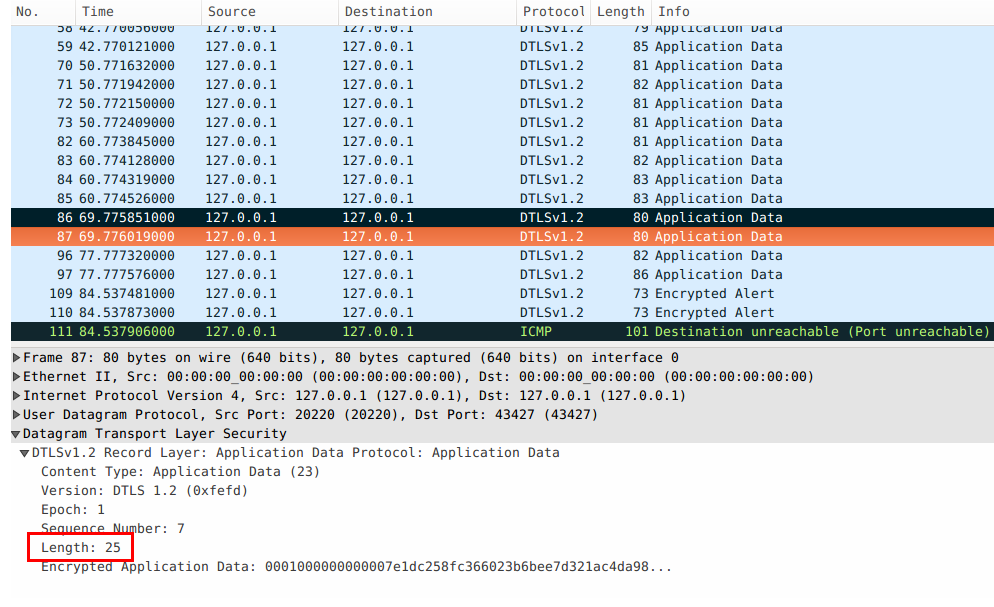
\includegraphics{./Pics/Wireshark01.png}}
\caption{Captured Leaky Coffee packets}
\label{Fig: Captured Packets 01}
\end{figure}

For example, a 2-packets session (packet No 86 and 87) has been marked out in \Cref{Fig: Captured Packets 01}. The values of DTLS Length  are both $25$ as marked in red rectangle. Their actual plaintext length can then be computed as $8$ and $8$ bytes respectively by \Cref{Eq: Plaintext length}. 

It is possible to do the single packet analysis described in \Cref{Sec: Guessing Plaintext by One Packet Length} on each of these packets. We immediately know that plaintext in the first packet is “ESPRESSO”; whilst the second one could be either “ESPRESSO” or “MOCHA” with a $Flavour$ of length $3$. However, the analysis of the second packet is in fact unnecessary at all as the application specifies that an “ESPRESSO” $Order$ can only be responded with an “ESPRESSO” with NULL $Flavour$.

The application specifies that the first part of the $Order||Flavour$ simply echoes the first packet; therefore in fact we can immediately tell that the second packet is “ESPRESSO”.
\end{example}

One way to model this is to “expand” the channel. Instead of using the content at each packet from as the input, we can write them as a vector:
\begin{equation*}
\vec{x} = <x_1, x_2, ..., x_n>
\end{equation*}

and similarly, we can also write their length as another vector:
\begin{equation*}
\vec{l} = <y_1, y_2, ..., y_n>
\end{equation*}

Then we can use the same strategy in \Cref{Sec: Guessing Plaintext by One Packet Length} to construct the leakage channel $W^{-1}(X, Y)$ where $\vec{x} \in X$ and $\vec{y} \in Y$. 

A problem in this method is the resulting channel is of the size of the Cartesian product of all contents in every packet. However, in this Leaky Coffee application most of the cells is actually $0$ which could be used to reduce its storage space; but such optimisation is heavily application dependant.

A probably better way to model this side channel is to use Hidden Markov Model\cite{baum1966} similar to \cite{Danezis_trafficanalysis}. Techniques of Machine Learning might also be able to utilise this side channel information more efficiently. However, in this “intentionally crafted” Leaky Coffee application, the first packet seems always enough to reveal (roughly) the rest of plaintext in a session.

\subsection{Estimate plaintext distribution}
In \Cref{Sec: Guessing Plaintext by One Packet Length} and \Cref{Sec: Guessing Plaintext Using Joint Packet Length} we have demonstrated how to construct a channel given the set of plaintext and their distribution. In this section, we will try to estimate the plaintext distribution by the distribution of ciphertext.

The general idea is that the distribution of length (as presented as $P$ column in \Cref{Tbl: Order3}) can actually be observed from the ciphertext; therefore we can revert the process and use it to estimate the distribution of plaintext.

\begin{example}
Assume we have a sample of encrypted $Order$ packet collected where we estimated the its length distribution as following: 
\begin{table}[H]
\begin{center}
{\begin{tabular}{|c|c|}
\hline
 $y$ & P     \\ \hline
5 & $d_1$ \\ \hline
8 & $d_2$ \\ \hline
9 & $d_3$ \\ \hline
\end{tabular}
}
\end{center}
\caption{Estimated length distribution from encrypted $Order$ packets}
\label{Tbl: Estimated length distribution from encrypted $Order$ packets}
\end{table}

Similar to \Cref{Exmp: Single-Order}, the first step is to construct a Content-Length channel. The difference is that this time we do not have the pre-knowledge of plaintext distribution; therefore we represent the content distribution as unknown variables $p_i$ for each content.

\begin{table}[H]
\begin{center}
{\begin{tabular}{c|l|l|l||l|}
$W(y|x)$          & 5 & 8 & 9 & $P$\\
\hline
"AMERICANO" &   &  & 1  & $p_1$ \\
\hline
"CAPPUCINO" &   &   & 1  & $p_2$\\
\hline
"MOCHA"     & 1 &   &    & $p_3$\\
\hline
"ESPRESSO"  &   &  1  &   & $p_4$\\
\hline
\end{tabular}
}
\end{center}
\caption{Content-Length Channel with unknown distibution of $Order$}
\label{Tbl: Content-Length Channel with unknown distibution of $Order$}
\end{table}


%Since we are only interested in $p_1$ and $p_3$ and the appearance of each content is exclusive, \Cref{Tbl: Content-Length Channel with unknown distibution of $Order$} can be rewritten as \Cref{Tbl: Rewritten Content-Length Channel with unknown distibution of $Order$}.
%
%\begin{table}[H]
%\begin{center}
%{\begin{tabular}{c|c|c|c||c|}
$W(y|x)$          & 5 & 8 & 9 & $P$\\
\hline
"AMERICANO" &   &  & 1  & $p_1$ \\
\hline
"MOCHA"     & 1 &   &    & $p_3$\\
\hline
"ESPRESSO" or "CAPPUCINO"  &   &  $p_4 / (p_2 + p_4)$  &  $p_2 / (p_2 + p_4)$  & $p_4 + p_2$\\
\hline
\end{tabular}
}
%\end{center}
%\caption{Rewritten Content-Length Channel with unknown distibution of $Order$}
%\label{Tbl: Rewritten Content-Length Channel with unknown distibution of $Order$}
%\end{table}

Their joint distribution follows immediately.

\begin{table}[H]
\begin{center}
{\begin{tabular}{c|c}

$\widehat{W}P$  & P     \\ \hline
("AMERICANO",9) & $p_1$ \\ \hline
("CAPPUCINO",9) & $p_2$ \\ \hline
("MOCHA",5)     & $p_3$ \\ \hline
("ESPRESSO",8)  & $p_4$ \\ \hline
\end{tabular}
}
\end{center}
\caption{Joint distribution of $(Order, l)$ with unknown distribution of $Order$}
\label{Tbl: Joint distribution of $(Order, l)$ with unknown distribution of $Order$}
\end{table}

Then we can compute the marginal distribution of length.

\begin{table}[H]
\begin{center}
{\begin{tabular}{|c|c|}
\hline
 $y$ & P     \\ \hline
5 & $p_3$ \\ \hline
8 & $p_4$ \\ \hline
9 & $p_1 + p_2$ \\ \hline
\end{tabular}}
\end{center}
\caption{Marginal distribution of $l$ with unknown distribution of $Order$}
\label{Tbl: Marginal distribution of $l$ with unknown distribution of $Order$}
\end{table}

By linking \Cref{Tbl: Marginal distribution of $l$ with unknown distribution of $Order$} with \Cref{Tbl: Estimated length distribution from encrypted $Order$ packets} we have the following constrains to the content distribution:

\begin{equation} \label{Eq: Plaintext Distribution Estimation}
\left\{
\begin{aligned}
p_3 = d_1\\
p_4 = d_2\\
p_1 + p_2 = d_3\\
\sum\limits_{i = 1}^4{p_i} = 1
}\right
\end{aligned}
\end{equation}

Any solution satisfies \Cref{Eq: Plaintext Distribution Estimation} can be viewed as a reasonable guess to the distribution of the contents.

\end{example}
